\documentclass{article}

\usepackage{amsmath}
\usepackage{mathtools}
\usepackage{amstext}
\usepackage{array}
\usepackage[long]{optidef}
\usepackage[backend=biber,
            url=false]{biblatex}
\usepackage{float}
\usepackage{tikz}
\usepackage{txfonts}
\usepackage[colorinlistoftodos]{todonotes}
\usepackage[long]{optidef}

  \addbibresource{ch1-2.bib}

  \usetikzlibrary{calc,matrix,decorations.markings,decorations.pathreplacing}
  \usetikzlibrary{positioning}

  \definecolor{colone}{gray}{0.7}
  \definecolor{coltwo}{gray}{0.6}
  \definecolor{colthree}{gray}{0.5}
  \definecolor{colfour}{gray}{0.9}
  \definecolor{colfive}{gray}{0.9}
  \definecolor{colsix}{gray}{0.9}
  \definecolor{colseven}{gray}{0.9}

  \tikzset{
  table/.style={
  matrix of nodes,
  row sep=-\pgflinewidth,
  column sep=-\pgflinewidth,
  nodes={rectangle,text width=2cm,align=center},
  text depth=1.25ex,
  text height=2.5ex,
  nodes in empty cells}
  }

  \tikzstyle{startstop} = [rectangle, minimum width=2cm, minimum height=1.5cm,text centered, draw=black]
  \tikzstyle{process} = [rectangle, minimum width=3cm, minimum height=1.5cm, text centered, draw=black]
  \tikzstyle{blank} = [circle, minimum width=0.1cm, minimum height=0.1cm, text centered, draw=white]
  \tikzstyle{arrow} = [thick,->,>=stealth]

\begin{document}

  \title{Chapter 2}

  \author{M. Repetto}

  \date{}

\maketitle

\begin{abstract}
  In the following paper is proposed a multi-objective model for components allocation in a Green Supply Chain framework. The model builds on the concept of the supply chain as suggested by Porter, and accounts for the costs of production using the Activity Based Cost accounting method (ABC). Such model is organized in blocks related to several moments in the value chain, from the procurement to the end customer. Above each and every one of these blocks, a series of environmental constraints have been included, and that the firm has to comply, with respect to specific country regulation, or in case of a particular Corporate Environmental Responsibility policy...\todo{to be continued when the model will be fully defined}
\end{abstract}

\section{Introduction}
  Global Supply Chain Management (GSCM) is probably one of the most used terms when the discussion of how the firms are running their business is brought to the table nowadays. GSCM may be defined as the allocation of goods and services along a series of transnational companies' global network to maximize profits and minimize waste. As the Supply Chain Professionals puts it, the goal of GSCM is threefold and focuses on delivering: (a)the right product; (b)to the right place; (c)at the right time.
  Inside this very wide paradigm, the concept of logistics serves as the backbone; recalling that logistics is developed to be in charge of the movement of goods, service and last but not least information from the sourcing of raw material, till it reaches the end customer.
  Along with these two concepts a third one sticks with them, the Green Supply Chain (GSC). This idea, brought to light by a more advanced concern about environmental matters of the developed countries, forced the firms to be accountable for their negative externalities related to the environment in which they operate \cite{srivastava_green_2007}.

  However such legislation lacks from a point of view of legal constraints, setting only a few qualitative restriction, poorly measurable by the enterprises or in some cases letting the customers pay for their environmental behavior toward waste disposition. These facts are inevitably leaving some degrees of freedom to the firms, on the other hand, is also important to notice that these are only seeds of legislation that show us how the long-term trend will be about the tolerance given to the behavior of firms with environmental concerns, a trend that in the future may require firms to set particular frameworks to be accountable for their environmental impact. Nowadays such effort is not achieved by the legal frameworks provided by the domestic legislators but by the Corporate Environmental Responsibility (CER), meaning that are the stakeholders to impose the companies to be more responsible on their day to day operations.

  Speaking about the literature, is observable an emerging branch which deals with the Green Supply Chain Management, a new paradigm of Supply Chain Management whose aim is to keep under control the behavior of the firm during its operations, by applying policies such as Green Manufacturing and Re-manufacturing, Green Design etc... Because of that a Goal Programming model is proposed, in order to address such problems; following what proposed by literature, an enhanced model is proposed, such model, fixing quantitative and qualitative constraints to the pollution generated by the value adding activities, involved in the creation of the good, tries to implement the benefits of a recycling program enacted by the firm apropos the WEEE directive. In the case under scope, the choice was to pick a networking electronic appliance business (i.e. hub, switch or router).  In order to measure such impact, a framework provided by the Activity Based Costing is used; such approach is used in order to assess and address the marginal environmental impact of any additional unit elaborated by the transnational firms.
\\
\\
The paper is organized in four parts where two of them are devoted to a review of the existing literature and the last two, which are a respectively model and result oriented. In the first of the literature sections a full overview of the Green Supply Chain framework will be given; at the same time the focus will be directed to the legal implications that are affecting both producer and distributors operating in the European Union. After this overview a deep analysis will be given on the state-of-the-art techniques used to model both Supply Chain Management and Logistics topics, focusing the attention on peculiar applications such as stochastic programming. Ultimately the two sections devoted to the model will be used to state the model proposed with its assumptions, and then to analyze its result through a scenario analysis.  


\pagebreak

\section{Green Supply Chain}
Green Supply Chain saw a steady growth of interest in many enterprises\cite{Diabat2011} as well as by academics; a growth that, looking to the data\cite{Strobel18}, reached its hype between the 2012 and 2014 (Figure \ref{fig:occurrence}) and that may be strengthen in the next years because of the increasing environmental concern. The main research fields interested by this phenomena are the ones involving environmental sciences, management, operational research and more generally green sustainable sciences\cite{Shan2018}  
\begin{figure}[ht]
	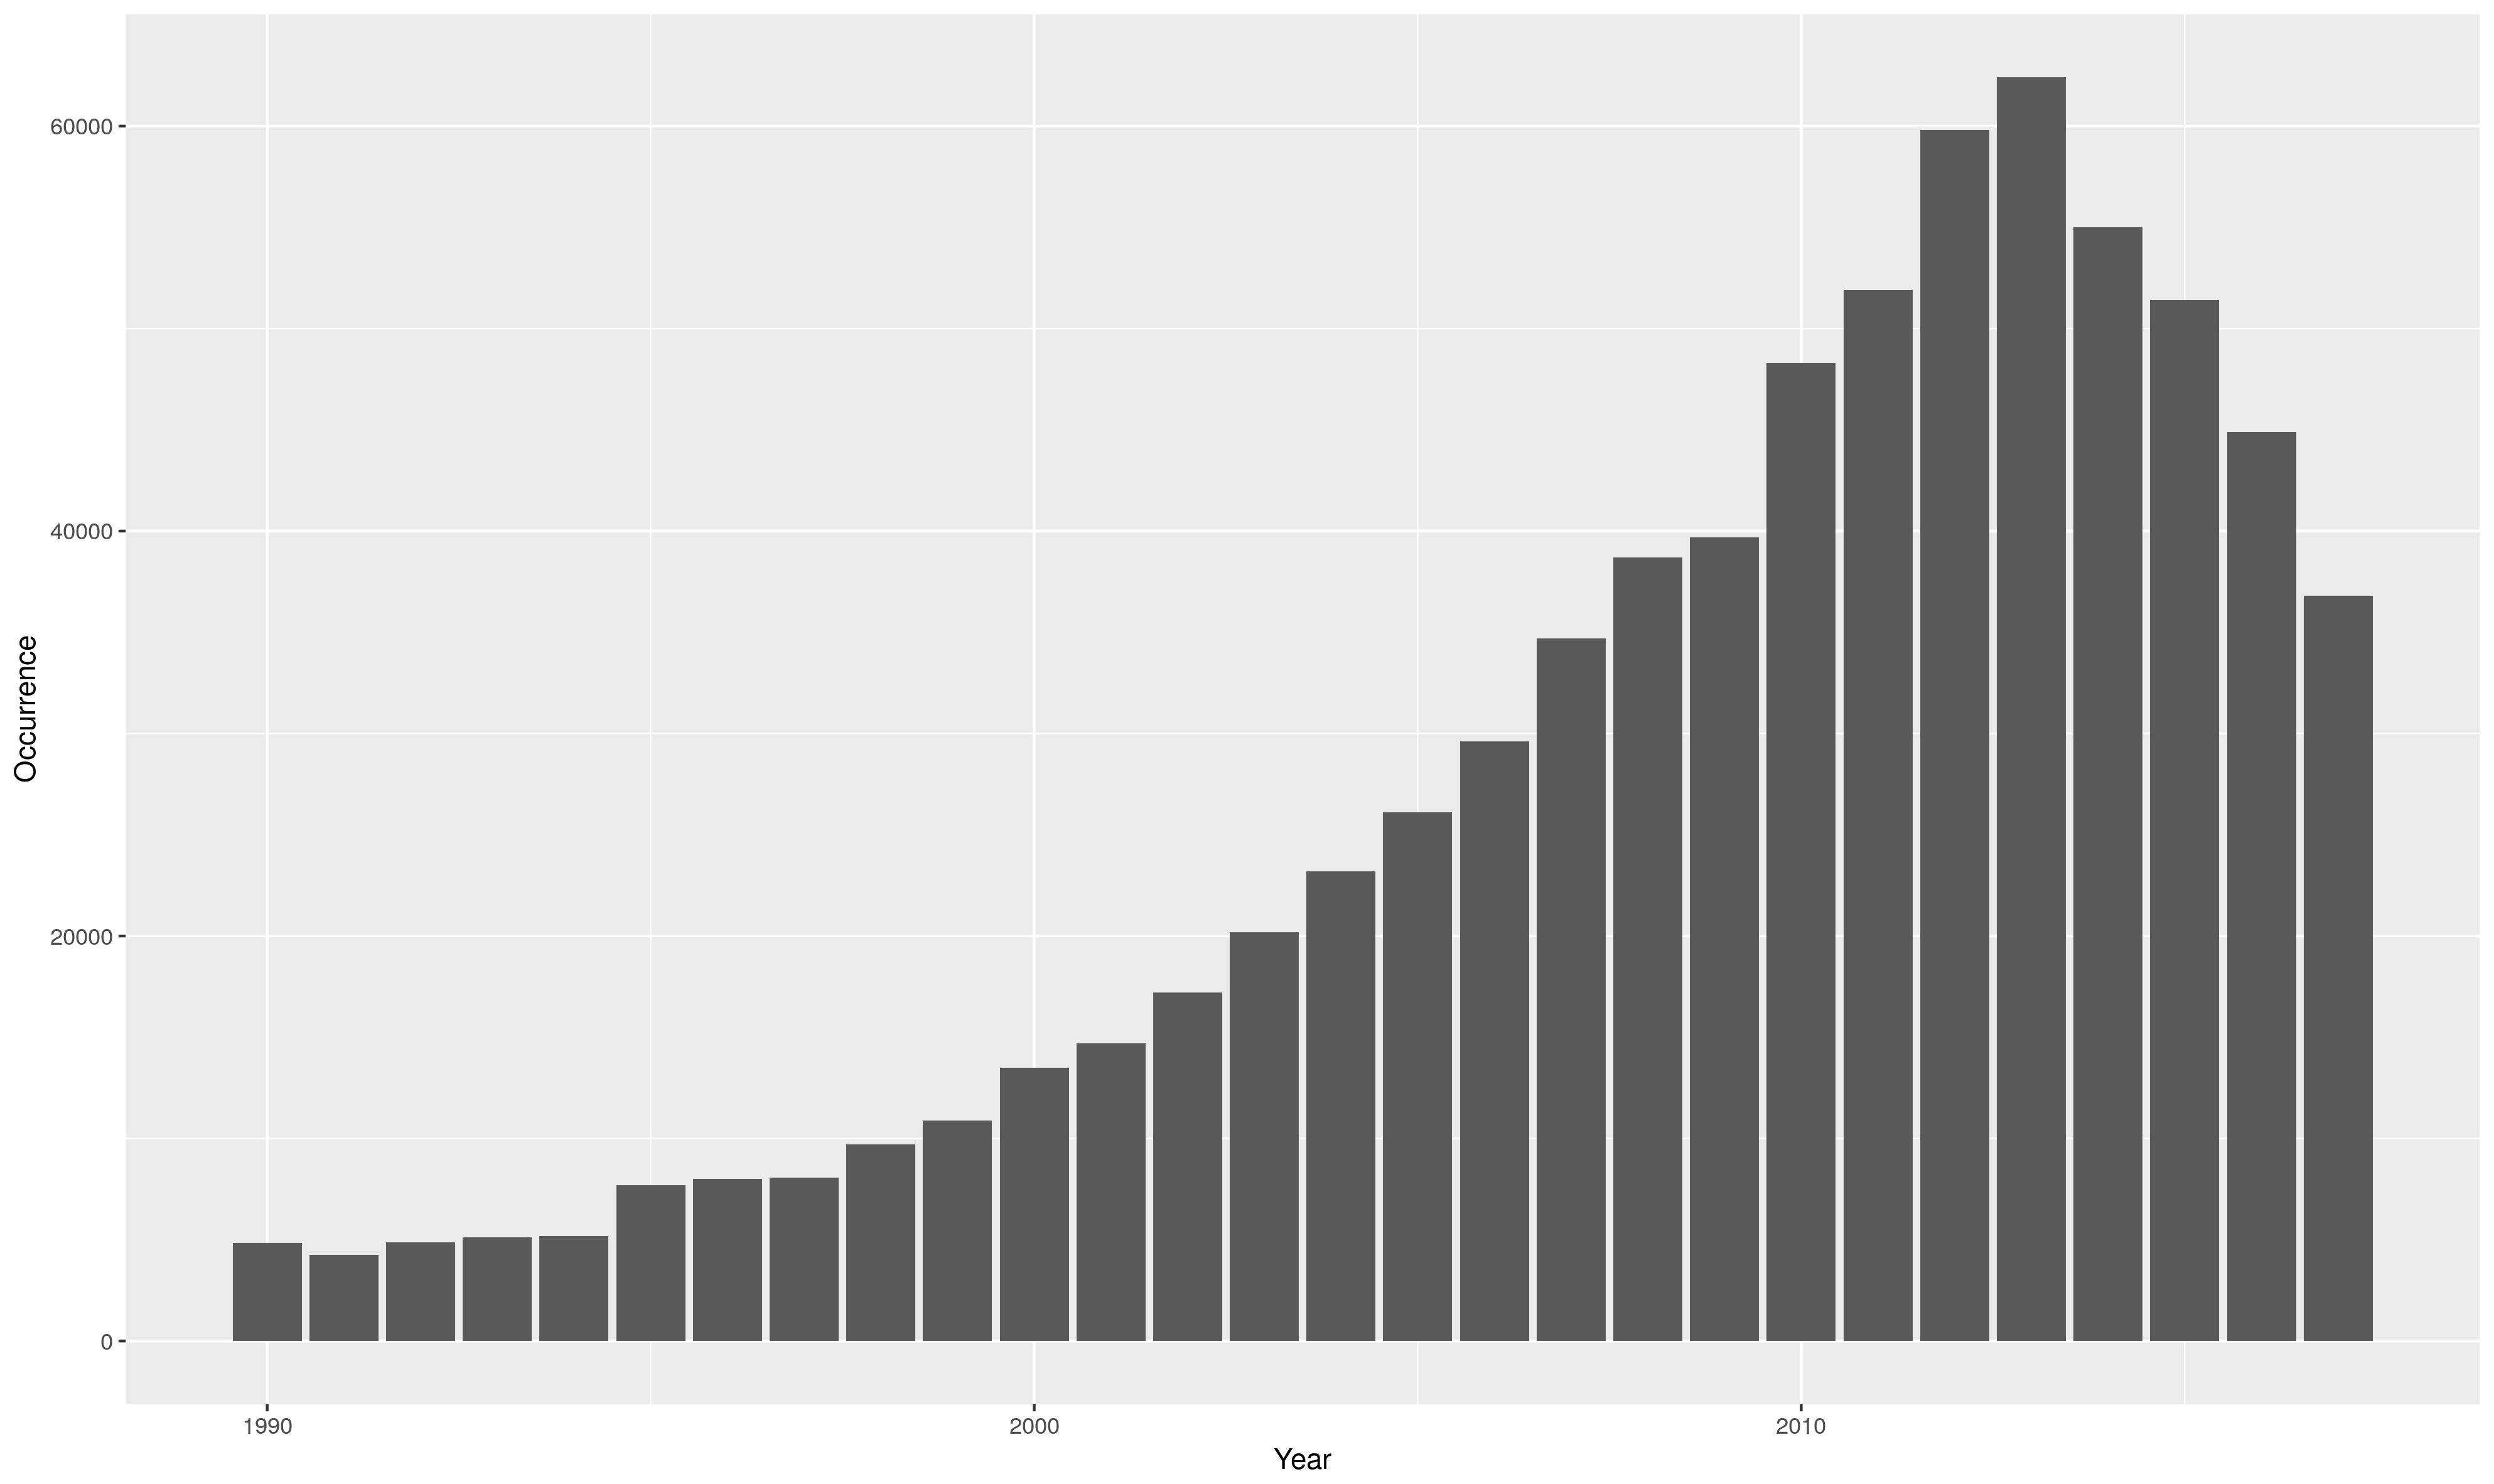
\includegraphics[width=\textwidth]{Images/occurence.png}	
	\label{fig:occurrence}
	\caption{Occurrence of Green Supply Chain in papers indexed by Google Scholar}	
\end{figure}
\\
Although Green Supply Chain manager is perceived as a game changer in order to unleash long term sustainability of a business, it's worth noting the lack of an univocal definition. In fact, some of the academics see GSCM as a process\cite{Gilbert2001}, more specifically a "greening process" from this school of thought belongs the line of thought that the management has the duty of incorporating the environmental criteria along all the organizational value creation process. Another definition sees the Green Supply Chain as a set of policies whose focus is to raise environmental concern along the production, distribution process\cite{Zsidisin2001}. In this paper we used a two level definition the first definition is a formal one that builds from the concept of Supply Chain Management as defined by the Council of Supply Chain Management Professionals; the second is a substantial and deals with the operations affecting the "green" practices inside the firm.
\\
In formal terms, Green Supply Chain may be defined as the series of interconnected activities across the border of different enterprises that adds value to the goods and services from the sourcing to the market. Its aim is to improve performance in measures of sustainability, cost reduction, emission reduction. Whereas Supply Chain Management sets its objectives to maximize profits and minimize waste, in economic terms, Green Supply Chain sets its objectives even further, posing as its ultimate mission to lower the ecological impact that a firm or a series of them has in their day to day operations. 
Such green operations\cite{srivastava_green_2007}\cite{Zhu2008} constitutes the substantial definition of Green Supply Chain Management, these operations are:
  \begin{itemize}
    \item Green Manufacturing and Re-manufacturing: is the process of controlling and reutilizing material in the manufacturing, in order to limit waste creation\cite{urvashi_green_2013};
    \item Green Design: is an approach put in place to promote the environmental quality of a certain product or service,  by reducing negative impacts on the natural environment; an example could be the automatic switch of the television after a period of idleness\cite{ceschin_evolution_2016}; and
    \item Green Operations in general: by green operation is intended any type of activity which does not fall into the two categories mentioned above but is characterized by a "green" attitude as for example the optimization of the offices consumption through a remote-working policy;
  \end{itemize}
  
  Apart from the definition and its importance in the business field is important to focus the attention of the main drivers affecting this change, in fact such drivers are many and involves the overall ecosystem of the firm (external drivers), and even the firm (internal drivers) in its reactions to this drivers plays a key role in setting its environmental behavior that may be reactive, focused, opportunistic, and proactive\cite{YolLee2007}. Speaking about the external drivers, they fall between four main categories:
  \begin{itemize}
	  \item Legal frameworks: embraces all the set of laws either soft or hard laws, that implies certain standards and regulation over the operations provided along the supply chain;
	  \item Customer relations and concerns: in this category pertain every possible action overtaken by the end-users who can force their pressure on the firm enacting non buying campaign and manifestation in general;
	  \item Supplier/distributors relations: the actions pertaining to this category are similar to the ones of the customers, the only difference is that since are enacted    by entities that are constituting the supply chain they can provoke major issue in providing good and services on the market;
	  \item External stakeholders, this category embraces all the stakeholders that do not follow in the categories of either customers and suppliers, which may include stockholder, agents involved by the environmental behavior of the firm, is an example the households living near the production plan, etc...
  \end{itemize}
Since the model proposed has it's aim in setting a Green Supply Chain network of products from the procurement sites to the end user market which has stated to be the Euro Zone; it's necessary to highlight the set of norms that characterizes such market and in particular a specific attention will be given to the norms concerning electrical products.

  \subsection{The legal framework: an European perspective}
  In the market under scope which is the European one, there are several legislation concerning the environmental impact of certain e-Products\footnote{for e-Products, is intended an electrical or electronic equipment such as computers, TV-sets, fridges, cell phones and other electronic appliances}. The most important are:
  \begin{itemize}
    \item Waste Electrical \& Electronic Equipment (WEEE);
    \item Restriction on Hazardous Substances (RoHS);and
    \item Ecodesign Requirement for Energy-using Product (EuP).
  \end{itemize}

  Such legal frameworks act at different levels from the sourcing to the customer involving community member States. The following flowchart illustrates this differences.

  \begin{figure}[ht]
    \centering

    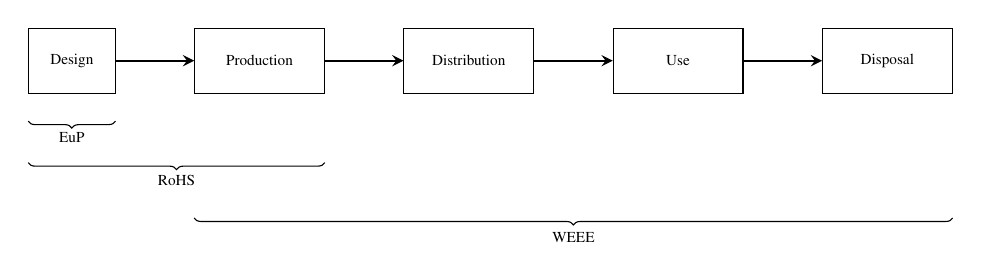
\begin{tikzpicture}[scale=0.8, every node/.style={scale=0.55}]
    \node (start) [startstop] {Design};
    \node (process1) [process, right=of start] {Production};
    \node (process2) [process, right=of process1] {Distribution};
    \node (process3) [process, right=of process2] {Use};
    \node (process4) [process, right=of process3] {Disposal};

    \draw [arrow] (start)--(process1);
    \draw [arrow] (process1)--(process2);
    \draw [arrow] (process2)--(process3);
    \draw [arrow] (process3)--(process4);

    \draw[decorate,decoration={brace,mirror,raise=10pt}]
    (start.south west) -- (start.south east) node[below, midway, yshift = -22]  {EuP};
    \draw[decorate,decoration={brace,mirror,raise=25pt}]
    (start.south west) -- (process1.south east) node[below, midway, yshift = -50]  {RoHS};
    \draw[decorate,decoration={brace,mirror,raise=45pt}]
    (process1.south west) -- (process4.south east) node[below, midway, yshift = -88]  {WEEE};

    \end{tikzpicture}
    \caption{Legislation affection}
  \end{figure}

  In the following subsection, an additional overview is given to such legislation.

\subsubsection{Waste Electrical \& Electronic Equipment}
  The Waste Electrical \& Electronic Equipment also called WEEE is ruled in the European Community by Directive 2002/96/EC now repealed by the Directive 2012/19/EU. The objectives of the policy are, to preserve, protect and improve the quality of the environment, to protect human health and to utilize natural resources prudently and rationally. That policy is based on the precautionary principle meaning that the polluter should pay for its damage. Is important to notice that in the European market such directive is impacting all the community members is not perfectly homogeneous ways because of the implementation which is remitted to the local authorities. This problem may incur in potential elusive behavior as highlighted by the German firms who exploited gaps in the law which have allowed them to move large amounts of WEEE declared for recycling to developing economies including India, China, Nigeria and Eastern Europe \cite{ongondo_how_2011}. Despite such cases, the overall impact of this directive is mostly positive as highlighted by the Eurostat data here exposed.

  The WEEE Directive currently sets a minimum collection target of 4 kg per year per inhabitant for WEEE from households. From 2016, the minimum collection rate shall be 45\% calculated on the basis of the total weight of WEEE collected. Where the WEEE is calculated with the following formula:
  $$
  W (n) = \sum{t = t_0}_{n} POM \cdot L^p(t,n)
  $$
  Where $W(n)$ refers to the specific quantity of electrical and electronic waste for a specific year, $POM(n)$ is the quantity of new electrical component injected in the market and $L$ is the discard-based lifespan profile for the electrical component injected in the market. From the graph proposed below is possible to see how the target of minimum collection of 4 kg per year per inhabitant for WEEE from households was achieved by all the countries in the Euro zone however not all the countries has the same collection rate, meaning that some of them may have introduced legislation that comply only with the minimum target of the directive, leaving the households with the freedom to dispose of their WEEE in unconventional manner. Clearly this means for the enterprises less obligations on the collection of e-Products, but at the same time less products to be recycled and less opportunity of remanufacturing.

  \begin{figure}
  \centering
  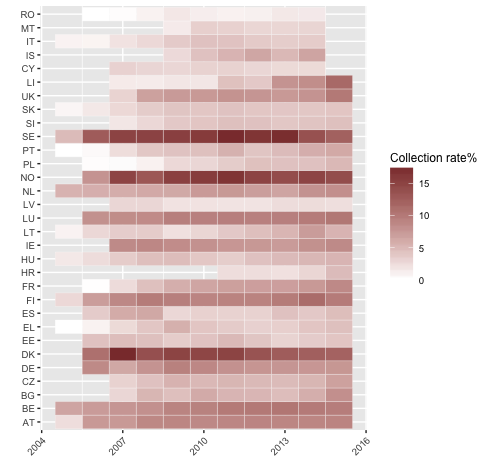
\includegraphics[width=0.8\linewidth]{Images/heatmap.png}
  \caption{Kilograms of WEEE collected per capita}
  \end{figure}

\subsubsection{Restriction on Hazardous Substances}
  The Restriction on Hazardous Substances also called RoHS is represented by the Directive 2017/2102 (RoHS 2 recast). The scope is the restriction on the use of certain hazardous substances in electrical and electronic equipment (EEE) such as lead, mercury, cadmium, hexavalent chromium etc... In such case, as opposed to the WEEE the RoHS directive acts as a barrier to the products containing such minerals and not when they become waste. In considering such regulation is worth noting that there are no differences between the dimension of the distributing entity, meaning that small businesses, as well as large businesses, are equally affected by these restrictions. The only amendment is given to the batteries that may exceed such restriction.

\subsubsection{Ecodesign Requirements for Energy-using Product}
  The Directive 2009/125/EC is meant to deal with Ecodesign regulations. Ecodesign regulations require manufacturers to decrease the energy consumption of their products by establishing minimum energy efficiency standards. In particular, The Ecodesign Directive provides a consistent legal framework for improving the environmental performance of products setting out a minimum mandatory requirement for the energy efficiency of these products. In case of the design of IT networking products such as routers and switches the firms are obliged by such directive to implement some ecodesign features such as the maximum wattage of 1W in case of off mode or a standby maximum consumption of 2W. Such measure per se do not impact in any case the supply chain since they are just additional features that has to be implemented in the products sold in Europe.

\pagebreak 

\section{A state-of-the-art review: mathematical modeling in SCM}
  As proposed by the Council of Supply Chain Management Professionals, the Supply Chain Management (SCM) is the planning and the management of all activities involved in sourcing and procurement, conversion, and logistics as well as coordination and collaboration with the entities. The problem arising from such activities seems to be well addressed by mathematical modeling, other advantages of such approach are the economic sustainability and the possibility to scale the model in order to address different situations.
  From the comprehensive review built by Muna et al. \cite{mula_mathematical_2010} the methods used by the academic world and the specific situations they tried to model, are:
  \begin{itemize}
	  \item Linear Programming: order quantity definition by means of decentralization\cite{jung_order_2008}, production and distribution planning taking into account country specific regulations\cite{Oh_Karimi_2006}, multiple points of sales planning\cite{Kanyalkar_2005};
	  \item Mixed Integer Linear Programming: network optimization and routing configuration\cite{romo_optimizing_2009}, distribution planning in an environment with just a production plant and many distribution centers\cite{Rizk_Martel2008};
    \item Non Linear Programming: optimization of production, transport and inventories\cite{benjamin_analysis_1989};
    \item Multi Objective Programming: replenishment production and distribution planning with conflicting objectives simultaneously\cite{torabi_interactive_2008}, master planning\cite{Chern_Hsieh_2007};
    \item Fuzzy Mathematical Programming: distribution allocation considering different products and production/distribution centers\cite{Liang_Cheng_2009};
    \item Stochastic Programming: addressing demand uncertainty accounting for the probability distribution\cite{Gupta_Maranas_2003};
    \item Heuristics Algorithms and Meta-Heuristics; and
    \item Hybrid Models.
  \end{itemize}

  Is worth noting how the majority of the models pertain to the category of Mixed Integer Linear Programming, this may be due to the fact that is probably one of the simplest and most reliable methods that can be used to solve such problems, however, this simplicity comes with some costs such as the focus on a single linear objective function with linear constraints whereas in reality different objectives has to be taken into account as for example the manager preferences toward greener choices. Another interesting topic brought into light by Aouni \cite{azimian_supply_2017} is that such models are generally deterministic, where in reality such assumption does not hold most of the time, for example, the demand forecast can't be deterministic at all and derives from a stochastic process. This lack of deterministic variable lies also in case of the procurement where the price of a commodity is said to follow a sort of stochastic process and an order may be placed several days after the decision make it.
  
  \subsection{Stochastic Optimization: a Goal Programming perspective}
  
  \subsection{Fuzzy Goal Programming}

  \pagebreak

\section{Model formulation}
The hybrid model developed is based on the supply chain concept developed by Santoso\cite{Santoso_Ahmed_Goetschalckx_Shapiro_2005}plus the integration of supporting activities as enunciated by Porter\cite{CompetitiveAdvantage}in his concept of value chain. Above the model, a fuzzy goal is created a fuzzy goal programming model that tries to capture the  DM preferences about the target collection rate that should be achieved by the company in order to foster sustainable operations and a Green Supply Chain.
The model proposed by Santoso is formulated as follow:

\begin{mini!}
	{y,x}{\sum_{i=1}^{P} c_i y_i  + \sum_{k=1}^{K} \sum_{(i,j)=1,1}^{A} q_{ij}^{k}x_{ij}^{k}}{}{}
	\addConstraint{\sum_{i=1}^{N} x_{ij}^k - \sum_{l=1}^{N} x_{jl}^k}{=0,}{\forall j \in P, \forall k \in K}
	\addConstraint{\sum_{i=1}^{N} x_{ij}^k}{\geq d_{j}^k,}{\forall j \in C, \forall k \in K}
\addConstraint{\sum_{j=1}^{N} x_{ij}^{k}}{\leq s_{i}^{k},}{\forall i \in L, \forall k \in K}
	\addConstraint{\sum_{k=i}^{K} r_{j}^k \cdot \sum_{i=1}^{N}x_{ij}^k}{\leq m_j y_i,}{\forall j \in P}
	\addConstraint{x \in \varmathbb{R}^+}{y \in Y[0,1]}{}
\end{mini!}

Where the objective function  is to minimize both the variable and fixed costs (here represented by the cost of building a plant) of a particular supply chain.
The constraint posed in $(1)$ serves to maintain the flow constant in each passage(so called flow conservation); the second and third constraint here represented by $(2)$ and $(3)$ are respectively controlling the volume of the demand (receiver side) and the supply (supplier side) of the supply chain; whereas the fourth constraint is used to control the capacity of each node. Lastly the $x$ variable, indicating the flow of goods to be positive and the variable $y$ indicating the effective construction of the plant to assume a value between 0 and 1. 
\\
It's worth noting that such model do not implement any support activities, whereas the Porter model mentions them. Therefore the hybrid model will contain a set of constraint indicating such activities and a new objective function embracing this change.

\begin{figure}
  \centering

  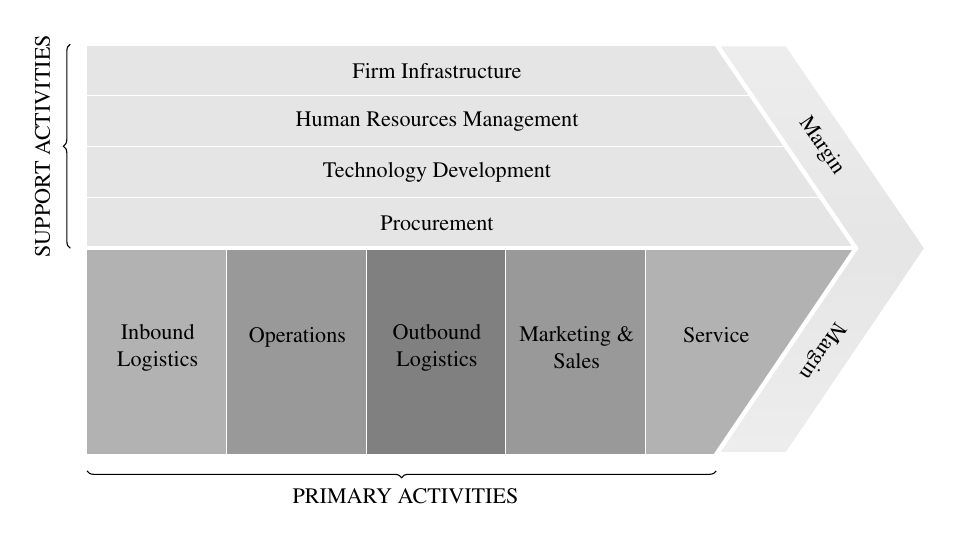
\begin{tikzpicture}[scale=0.8, every node/.style={scale=0.8}]
  \matrix (mat) [table]
  {
  |[fill=colfour]| & |[fill=colfour]| & |[fill=colfour]| & |[fill=colfour]| & |[fill=colfour]| &  \\
  |[fill=colfive]| & |[fill=colfive]| & |[fill=colfive]| & |[fill=colfive]| & |[fill=colfive]| &  \\
  |[fill=colsix]| & |[fill=colsix]| & |[fill=colsix]| & |[fill=colsix]| & |[fill=colsix]| & |[fill=colsix]| \\
  |[fill=colseven]| & |[fill=colseven]| & |[fill=colseven]| & |[fill=colseven]| & |[fill=colseven]| & |[fill=colseven]| \\
  |[fill=colone]| & |[fill=coltwo]| & |[fill=colthree]| & |[fill=coltwo]| & |[fill=colone]| & |[fill=colone]|  \\
  |[fill=colone]| & |[fill=coltwo]| & |[fill=colthree]| & |[fill=coltwo]| & |[fill=colone]| & |[fill=colone]|  \\
  |[fill=colone]| & |[fill=coltwo]| & |[fill=colthree]| & |[fill=coltwo]| & |[fill=colone]| & \\
  |[fill=colone]| & |[fill=coltwo]| & |[fill=colthree]| & |[fill=coltwo]| & |[fill=colone]| &  \\
  };

  \foreach \row in {2,3,4}
  \draw[white] (mat-\row-1.north west) -- (mat-\row-6.north east);
  \draw[white,ultra thick] (mat-1-1.north west) -- (mat-1-6.north east);
  \draw[white,ultra thick] (mat-5-1.north west) -- (mat-5-6.north east);

  \foreach \col in {2,3,4,5}
  \draw[white] (mat-5-\col.north west) -- (mat-8-\col.south west);

  \node[fill=colfour] at (mat-1-3) {Firm Infrastructure};
  \node[fill=colfive] at (mat-2-3) {Human Resources Management};
  \node[fill=colsix] at (mat-3-3) {Technology Development};
  \node[fill=colseven] at (mat-4-3) {Procurement};
  \node at ([yshift=-10pt]mat-6-1) {\parbox[t]{2cm}{\centering Inbound Logistics}};
  \node at ([yshift=-10pt]mat-6-2) {\parbox[t]{2cm}{\centering Operations \\\mbox{}}};
  \node at ([yshift=-10pt]mat-6-3) {\parbox[t]{2cm}{\centering Outbound Logistics}};
  \node at ([yshift=-10pt]mat-6-4) {\parbox[t]{2cm}{\centering Marketing \& Sales}};
  \node at ([yshift=-10pt]mat-6-5) {\parbox[t]{2cm}{\centering Service \\\mbox{}}};
  \node[rotate = 90] at ([xshift=-52pt]mat-3-1.north) {SUPPORT ACTIVITIES};
  \node at ([yshift=-19pt,xshift=-0.5cm]mat-8-3.south) {PRIMARY ACTIVITIES};

  \fill[white] (mat-1-5.north east) -- (mat-5-6.north east) -- (mat-1-6.north east) -- cycle;
  \fill[white] (mat-8-5.north east) -- (mat-5-6.north east) -- (mat-8-6.north east) -- cycle;

  \shade[top color=colfour!70,bottom color=colfour!70,middle color=colseven,draw=white,ultra thick]
  (mat-1-5.north) -- (mat-5-6.north) -- (mat-8-5.south) --
  (mat-8-5.south east) -- (mat-5-6.north east) -- (mat-8-5.south east) --
  (mat-5-6.north east) -- (mat-1-5.north east) -- cycle;

  \begin{scope}[decoration={markings,mark=at position .5 with \node[transform shape] {Margin};}]
  \path[postaction={decorate}]
  ( $ (mat-1-5.north)!0.5!(mat-1-5.north east) $ ) -- ( $ (mat-5-6.north)!0.5!(mat-5-6.north east) $ );
  \path[postaction={decorate}]
  ( $ (mat-5-6.north)!0.5!(mat-5-6.north east) $ ) -- ( $ (mat-8-5.south)!0.5!(mat-8-5.south east) $ );
  \end{scope}

  \draw[decorate,decoration={brace,mirror,raise=6pt}]
  (mat-1-1.north west) -- (mat-5-1.north west);
  \draw[decorate,decoration={brace,mirror,raise=6pt}]
  (mat-8-1.south west) -- (mat-8-5.south);
  \end{tikzpicture}

  \caption{Porter's Value Chain}
\end{figure}

Such activities are a fundamental part on the supply chain that serves as glue with the supply chain steps to the deliver the value to the end-customer. Therefore the hybrid model will looks like this:

\begin{mini}
  {w,u}{f(w)+ R(w+6x)+ H(100w-x*w/500)}{}{}
  \breakObjective{-g(w^3-x^2*200+10000*w^5)}
  \addConstraint{g(w_k)+h(w_k)}{=0,}{k=0,\ldots,N-1}
  \addConstraint{l(w_k)}{=5u,\quad}{k=0,\ldots,N-1}
\end{mini}

\begin{equation*}
\begin{aligned}
	min \sum_{k=1}^{K} \sum_{(i,j)=1,1}^{A} q_{ij}^{k}x_{ij}^{k} + \sum_{i=1}^{P^\star} c_i q_i \sum_{k=1}^{K} \sum_{(i,j)=1,1}^{A}x_{ij}^{k} 
\\
  \text{Subject to}
\\
\end{aligned}
\end{equation*}
\begin{equation}
  \sum_{i=1}^{N} x_{ij}^k - \sum_{l=1}^{N} x_{jl}^k = 0 \quad \forall j \in P, \forall \in K
\end{equation}
\begin{equation}
  \sum_{i=1}^{N} x_{ij}^k \geq d_{j}^k \quad \forall j \in C, \forall k \in K,
\end{equation}
\begin{equation}
  \sum_{j=1}^{N} x_{ij}^{k} \leq s_{i}^{k}  \quad \forall i \in L, \forall k \in K,
\end{equation}
\begin{equation}
	\sum_{k=i}^{K} r_{j}^k \cdot \sum_{i=1}^{N}x_{ij}^k \leq m_j y_i \quad \forall j \in P,
\end{equation}
\begin{equation}
\sum_{i=1}^{N^\star} q_{i}^j = n_j \quad \forall j \in P,
\end{equation}
\begin{equation}
  x \in \varmathbb{R}^+ \quad \quad 
  y \in Y[0,1] \quad \quad  q \in Q[0,1]
\end{equation}

In formulating our hybrid model is not taken into account the fixed cost of building a plant, this happened for two reasons. The first reason is the consideration of the cost of building a plant as a sunk cost and therefore it should not influence the economic decision on whether to allocate a particular quantity of goods on a specific plant. Secondly, because the Activity Based Cost method is used the focus will be on the activities that contributes in creating the marginal cost of the good in the supply chain. 

Finally the  implementation of the concept of green supply chain from a point of view of the legislation activated by the EU countries. However since such legislation, especially the WEEE does not impose any quantifiable level to be collected by the firms but is intended to be for the ultimate polluters (meaning the end customers) is necessary a way to proxy the potential of collection of each country in order to forecast the collected quantity that the firm expect to receive each year on the base of what is sold today. Because the electronic waste turns out to be a resource for the firm is necessary to model the fuzziness of such desire expressed by the DM, and therefore the implementation of a Fuzzy set\cite{Zadeh_1965} defined as:
$$
\mu [f_q(x)]=
\begin{cases}
1 & f_q(x) \geq b_q \\
1-\frac{b_q-f_q(x)}{n_{max}} & b_q -n{max} \leq f_q(x) \leq b_q \\
0 & f_q(x) \leq b_q - n_{max}
\end{cases}
$$
Such set penalized the negative deviations from the target demanded by the decision maker. In our case the \textit{ratio} behind this is given by the fact that a very low amount of collected electrical waste may turn out as higher cost of production because of the additional cost of buying new material. Conversely is also important to take


\subsection{The Goal Programming model}
Since the goals of the problem stated before are trying to model a set of different objectives the choices was to opt for the Goal Programming as a multi-criteria analysis tool therefore the resulting model will be set as follow: 
\\
The model proposed takes into account only one commodity because of simplicity matters however it can be adjusted to allow more than one commodity by including the transformation process of each production step. The additional rules to be implemented in the model may derive from other supply chain management tool more focused on the operational level such as production tree, etc... An example of such integration is proposed below.

In this case is possible to see how the two initial commodities are transformed passing through the production stage in one product that from now on will be used in the model for all the additional processes. From such simple example is evident that the process of transformation creates less goods passing from a stage to another, conversely the opposite contradict the production tree assumptions and therefore will not be taken into account. 

\subsubsection{Objective function}
The objective function that has to be minimized contains all the deviation from the soft constraints contained in equations ... 
\subsubsection{Constraints}
The hard constraints identified by the equations from ... to ... are summarized below 

\pagebreak

\section{Results and Conclusion}
In order to test such model a fictitious example is proposed by... Since some more assumptions were included as well as constraints compared to what proposed by the author, such as the fuzzy goal in maintaining a target level of electrical waste collection) additionally some some rules where implemented when defining the additional data, such rules are:
\begin{itemize}
	\item
	\item
\end{itemize}


\newpage 

\printbibliography

\end{document}
